\documentclass[9pt]{beamer}
\usepackage{kotex}
\usepackage{amsfonts,amssymb,amsthm}
\usepackage[dvipsnames]{xcolor}
\usepackage{xcolor}
\usepackage{etoolbox}
\usepackage{braket}
\usepackage{qcircuit}

%## color
\definecolor{customBlack}{HTML}{3B4252}
\definecolor{customBlackGrey}{HTML}{434C5e}
\definecolor{cuatomGrey}{HTML}{4C566A} 
\definecolor{customWhite}{HTML}{ECEFF4} 
\definecolor{customBlue}{HTML}{6082B6}  
\definecolor{customRed}{HTML}{BF616A}
\definecolor{vividauburn}{rgb}{0.58, 0.15, 0.14}


%## Theme & custom
% \usetheme{metropolis}           % Use metropolis theme
% \metroset{block=fill}
\usetheme{moloch} % modern fork of the metropolis theme
\molochset{block=fill}
\setbeamersize{text margin left=5mm, text margin right=5mm}
\setbeamercolor{palette primary}{bg=customBlack}
\setbeamercolor{alerted text}{fg=customRed}
\setbeamercolor{itemize item}{fg=customBlue}
\setbeamercolor{enumerate item}{fg=customBlue}


%## font
\usefonttheme[onlymath]{serif}
% \setbeamerfont{normal text}{size=\small}
% \setbeamerfont{math text}{size=\tiny}


%## Theorem title, numbering
\makeatletter
\setbeamertemplate{theorem begin}
{%
\begin{\inserttheoremblockenv}
{%
\inserttheoremheadfont
\inserttheoremname
\ifx\inserttheoremaddition\@empty\else\ of\ \inserttheoremaddition\fi%
\inserttheorempunctuation
}%
}
\setbeamertemplate{theorem end}{\end{\inserttheoremblockenv}}
\makeatother
\setbeamertemplate{theorems}[numbered]  


%## Custom block
\setbeamercolor{block title}{bg=customBlue, fg=white}
\setbeamercolor{block body}{bg=customWhite, fg=customBlack}
\setbeamercolor{block title alerted}{%
    use={block title, alerted text},
    bg=customRed,
    fg=white
}
\setbeamercolor{block body alerted}{%
    use={block title, alerted text},
    bg=customWhite,
    fg=customBlack
}
\AtBeginEnvironment{definition}{%
    \setbeamercolor{block title}{fg=white,bg=customBlackGrey}
    \setbeamercolor{block body}{fg=customBlack, bg=customWhite}
}
\AtBeginEnvironment{theorem}{%
    \setbeamercolor{block title}{fg=white,bg=customBlackGrey}
    \setbeamercolor{block body}{fg=customBlack, bg=customWhite}
}
\AtBeginEnvironment{corollary}{%
    \setbeamercolor{block title}{fg=white,bg=customBlackGrey}
    \setbeamercolor{block body}{fg=customBlack, bg=customWhite}
}
\AtBeginEnvironment{lemma}{%
    \setbeamercolor{block title}{fg=white,bg=customBlackGrey}
    \setbeamercolor{block body}{fg=customBlack, bg=customWhite}
}


%! Useful command
\renewcommand{\Pr}{\text{Pr}}
% $\ast$ \underline{Proof}:
%\checkmark \underline{meaning}:

\title{3. General Quantum Dynamics for Error correction}
\date{\today}
\author{Vaughan Sohn}
% \institute{Centre for Modern Beamer Themes}


\begin{document}
    %#################################### 
    \maketitle
    
    %#################################### 
    \begin{frame}
        \frametitle{Contents}
        \tableofcontents
    \end{frame}

    %#################################### 
    \begin{section}{General Quantum Dynamics}
        \begin{frame}
            \frametitle{Motivation}
            
            
            \begin{itemize}
                \item 이상적인 quantum dynamic에서는 완벽하게 외부와 상호작용하지 않는 closed system을 고려할 수 있다. 
                \item 그러나 실제 현실 세계에서는 environment나 ancilla bits등과 원하지 않는 상호작용이 발생하고, 그 결과로 \alert{noise}가 나타난다.
                \vspace{0.4cm}
                \item open quantum system을 다뤄야 하는 2가지 motivation:
                \begin{itemize}
                    \item Measurement outcome을 이용한 system의 control
                    \item Environment의 noise를 분석
                \end{itemize}
            \end{itemize}
            \begin{columns}
                \begin{column}{0.5\textwidth}
                    \begin{table}[h]
                        \[
                        \begin{array}{c}
                        \Qcircuit @C=1em @R=.8em {
                            \lstick{\rho } & \qw   &  \gate{U} & \qw & \rstick{U \rho U^\dagger} \qw \\
                        }
                        \end{array}
                        \]
                        \caption{closed system}
                    \end{table}
                \end{column}
                \begin{column}{0.5\textwidth}
                    \begin{table}[h]
                        \[
                        \begin{array}{c}
                        \Qcircuit @C=1em @R=.8em {
                            \lstick{\rho } & \qw  &   \multigate{1}{U}  & \qw &\rstick{\varepsilon(\rho)} \qw \\
                            \lstick{\rho_{\operatorname{env}} } & \qw  &   \ghost{U}  & \qw &\qw \\
                        }
                        \end{array}
                        \]
                        \caption{open system} 
                    \end{table}
                \end{column}
            \end{columns}
        \end{frame}

        \begin{frame}
            \frametitle{Motivation}
            
            Example: environment noise
            \vspace{0.2cm}
            \begin{itemize}
                \item $\ket{0}$ state에 unitary gate $X$를 가하는 연산을 가정하자.
                \item closed system에서는 100\% 확률로 측정결과 $1$을 얻게 된다.
                \item 그러나 open system에서는 environment가 원하지 않는 상호작용을 수행하여 $X$ gate가 정상적으로 가해지지 않을 수 있다.
                \item 최종 state는 우리가 원하는 state와 원치않는 state의 mixed state가 된다.
                $$ \rho = (1-p) \ket 0 \bra 0 + p X\ket 0 \bra 0 X^\dagger $$
                \item 따라서 open system의 outcome은 각각 다음의 확률을 가지고 관측된다.
                    \begin{itemize}
                        \item $p(0) = 1-p$
                        \item $p(1) = p$
                    \end{itemize}
            \end{itemize}
            \begin{columns}
                \begin{column}{0.45\textwidth}
                    \begin{table}[h]
                        \[
                        \begin{array}{c}
                        \Qcircuit @C=1em @R=.8em {
                            \lstick{\ket{0}} & \qw   &  \gate{X} & \meter & \rstick{1} \qw \\
                        }
                        \end{array}
                        \]
                        
                    \end{table}
                \end{column}
                \begin{column}{0.55\textwidth}
                    \begin{table}[h]
                        \[
                        \begin{array}{c}
                        \Qcircuit @C=1.1em @R=1.2em {
                            & & & &\lstick{\sqrt{1-p} \ket{0} + \sqrt p \ket{1}}  & \qw  &   \ctrl{1}  & \qw & \qw \\
                            & & & &\lstick{\ket{0}} & \qw  &   \gate{X}  & \meter & \rstick{?} \qw \\
                        }
                        \end{array}
                        \]
                    \end{table}
                \end{column}
            \end{columns}

        \end{frame}

        \begin{frame}
            \frametitle{General Quantum Dynamics}
            이제 general quantum dynamics를 표현하는 방법을 정의해보자.
            \begin{itemize}
                \item $\rho_{\operatorname{env}}$가 처음에 $\ket 0 \bra 0$ state로 준비되었고 $\{\ket i\}$를 env의 basis라고 하자.
                \item Environment는 우리의 측정 대상이 아니기 때문에, 최종 state $\varepsilon (\rho)$는 system에 대한 reduced state로 정의한다.
                \item Kraus operator $K_i \triangleq \braket{i | U | 0}$ 는 system에 대한 operator이다. 
                \begin{align*} \varepsilon (\rho) &=  \text{tr}_E \big( U(\rho \otimes \ket 0 \bra 0 )U^\dagger \big) \\ 
                    &= \sum_i \braket{i|U (\rho \otimes |0}\braket{0|) U^\dagger |i} 
                    \\ &= \sum_i \underbrace{\braket{i|U|0}}_{K_i} \rho \braket{0|U^\dagger |i} \\ &= \sum_i K_i \rho K_i^\dagger  \quad \leftarrow \text{operator-sum representation}\end{align*}
            \end{itemize}
            \vspace{-0.4cm}
            \begin{table}[h]
                \[
                \begin{array}{c}
                \Qcircuit @C=1em @R=.8em {
                    \lstick{\rho } & \qw  &   \multigate{1}{U}  & \qw &\rstick{\varepsilon(\rho)} \qw \\
                    \lstick{\rho_{\operatorname{env}}  = \ket{0} \bra{0}} & \qw  &   \ghost{U}  & \qw &\qw \\
                }
                \end{array}
                \]
            \end{table}
            \vspace{-0.6cm}
        \end{frame}

        \begin{frame}
            \frametitle{General Quantum Dynamics}
            이제 general quantum dynamics를 표현하는 방법을 정의해보자.
            \begin{itemize}
                \item General quantum dynamics는 각각의 kraus operator들이 system에 연산한 결과들의 합으로 표현할 수 있다.
                $$ \varepsilon (\rho) = \sum_i K_i \rho K_i^\dagger  \quad \leftarrow \text{operator-sum representation}$$
                \item Kraus operator들은 completeness relation을 만족한다. (system에 대해서)
                \begin{align*} \sum_i K_i ^\dagger K_i 
                    &= \sum_i \braket{0|U^\dagger |i} \braket{i|U | 0} \\ &= \braket{0|U^\dagger(\underbrace{\Sigma_i \ket i \bra i}_{I_E}) U |0} \\ &= \braket{0|\underbrace{U^\dagger U}_{I_{SE}}|0} = I_S\end{align*}
            \end{itemize}
        \end{frame}

        \begin{frame}
            \frametitle{Represent system by General Quantum Dynamics}
            \begin{itemize}
                \item Ancilla bits를 사용하는 system을 생각해보자. (e.g., phase estimation $\ket u$)
                \begin{figure}
                    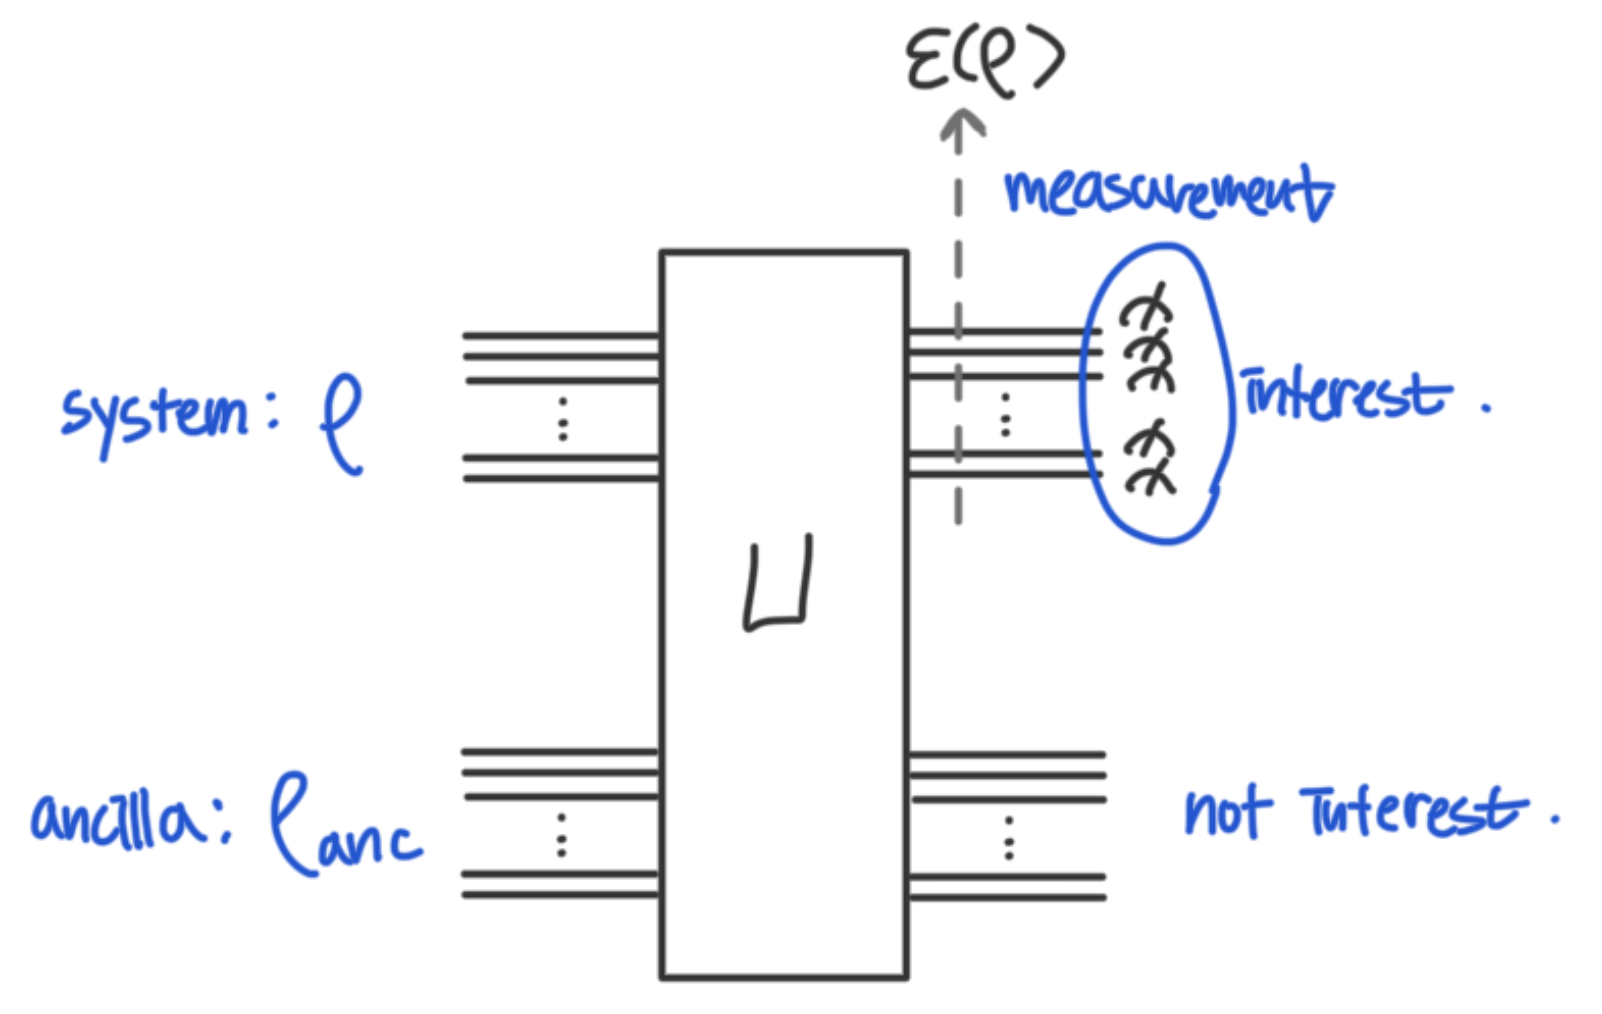
\includegraphics[width=0.45\textwidth]{image/L3_ancilla.png}
                \end{figure}
                \item composite system의 최종 상태는 다음과 같이 전개할 수 있다. (tip: $I_A$를 곱해준다.)
                \begin{align*} U\ket{\psi_S} \ket{0_A} &= I_A U \ket{\psi_S} \ket{0_A}
                    \\ &= \sum_i \ket{i_A} \bra{i_A}U \ket{\psi_S} \ket{0_A} \\ &= \sum_i \ket{i_A} \underbrace{\braket{i_A|U|0_A}}_{K_i} \ket{\psi_S} \\ &= \sum_i K_i \ket{\psi_S} \ket{i_A}\end{align*}
            \end{itemize}
        \end{frame}

        \begin{frame}
            \frametitle{Represent system by General Quantum Dynamics}
            \begin{itemize}
                \item system의 최종상태를 관찰하면, ancilla bits에 대한 state인 $\ket{i_A}$와 system에 대한 state인 $K_i \ket{\psi_S}$로 이루어진다는 것을 알 수 있다.
                $$ U \ket{\psi_S} \ket{0_A} = \sum_i K_i \ket{\psi_S} \ket{i_A}$$
                \item 그러나, 최종 상태는 현재 superposition state이기 때문에 $K_i$중에서 실제로 어떤 operator가 system에 적용되는지는 알 수 없다.                    
            \end{itemize}
            \vspace{0.2cm}
            \begin{block}{Idea}
                \textbf{Ancilla bits를 측정}하면, kraus operator가 의존하는 eigenvector $\ket{i_A}$가 무엇인지를 알 수 있기 때문에, system에 가해진 operator가 무엇인지를 알아낼 수 있다! 
            \end{block}
            \vspace{0.2cm}
            $\rightarrow$ 이는 실제로 quantum error detection의 기본 아이디어이기도 하다.
        \end{frame}
    \end{section}

    %#################################### 
    \begin{section}{Quantum Error Detection}
        \begin{frame}
            \frametitle{Idea of Quantum error detection}
            \begin{itemize}
                \item Quantum error의 원인은 대부분 environment이다.
                \item General quantum dynamics 표현에 의하면, env/anc의 state를 측정하여 얻은 $\ket i$로부터 system에 가해진 operator $K_i$가 무엇인지 알 수 있다.
                \item 따라서 $K_i$가 원래 우리가 system에 취하려고 했던 연산인지 아닌지를 확인하여 error를 detection할 수 있다.
                \vspace{0.5cm}
                \item \underline{Problem}: 그러나 environment는 우리가 직접적으로 측정할 수 없다.
                \item \underline{Solution}: environment 대신 우리가 측정할 수 있는 ancilla bits를 추가하자!
            \end{itemize}
        \end{frame}

        \begin{frame}
            \frametitle{Quantum error detection algorithm}
            \begin{itemize}
                \item 주어진 quantum circuit의 composite system은 단계별로 다음과 같이 변한다.
                \begin{enumerate}
                    \item $I \otimes C(X)$:
                    $$\left( \sqrt{1-p} \ket 0 + \sqrt p \ket 1 \right)\left( \alpha \ket{00} + \beta \ket{11} \right)$$
                    \item $C(X) \otimes I$:
                    $$\Big( \sqrt{1-p} \ket 0(\alpha\ket{00} + \beta \ket{11} \Big) +  \Big(\sqrt p \ket 1 (\alpha \ket{10} + \beta \ket{01}) \Big)$$
                    \item measurement: 만약 sys = anc이면 $X^2 = I$라서 state가 $\ket 0$이지만 sys $\ne$ anc이면 $X$이라서 $\ket 1$이 된다.
                    $$\begin{cases} 0, & \alpha \ket{00} + \beta \ket{11} \\ 1, & \alpha \ket{01} + \beta \ket{10} \end{cases} $$
                \end{enumerate}
                \vspace{0.2cm}
                \item system qubit과 ancilla qubit이 동일한 경우엔 측정 결과가 $0$이 되고 다른 경우에는 측정결과가 $1$이 된다. $\rightarrow$ error가 발생했음을 감지할 수 있다.
            \end{itemize}
            \vspace{-0.4cm}
            \begin{table}[h]
                \[
                \begin{array}{c}
                \Qcircuit @C=1.5em @R=1em {
                    & & & & & & \lstick{\text{Env : } \sqrt{1-p}\ket 0 + \sqrt p \ket 1}  & \qw \barrier[-1.3em]{2}   &\ctrl{1} \barrier[-1.1em]{2}   &\qw  &  & \\
                    & & & & & & \lstick{\text{Sys : } \alpha \ket{0} + \beta \ket 1}      & \ctrl{1}                  &\targ                          &\ctrl{2}       &   & \\
                    & & & & & & \lstick{\text{Anc : } \ket{0}}                            & \targ                     &\qw                            &\qw        &  \ctrl{1}    & \\
                    & & & & & & \lstick{\ket 0}                                           & \qw                       &\qw                            &\targ   &  \targ \barrier[-1.7em]{0}     & \meter
                }
                \end{array}
                \]
            \end{table}
            \vspace{-0.4cm}
        \end{frame}
    \end{section}
    
    %#################################### 
    \begin{frame}{References}
        
        \begin{itemize}
            \item Lecture notes for EE547: Introduction to Quantum Information Processing (Fall 2024)
        \end{itemize}
        \vspace{6cm}
    \end{frame}

\end{document}